\documentclass[12pt]{article}

\usepackage{fullpage}
\usepackage{graphicx}
\usepackage{graphics}
\usepackage{mdwlist}
\usepackage{amsmath}
\usepackage{bm}


% christos: these look closer to NSF specs\dots
\setlength{\oddsidemargin}{0.0in}
\setlength{\evensidemargin}{0.0in}
\setlength{\textwidth}{6.5in}
\setlength{\headheight}{0.0in}
\setlength{\topmargin}{0.0in}
% \setlength{\textheight}{9.0in}
\setlength{\textheight}{9in}
\addtolength{\textheight}{-\topmargin}
\addtolength{\textheight}{-\headheight}
\addtolength{\textheight}{-\headsep}
\addtolength{\textheight}{-\footskip}

\begin{document}

\newcommand{\beq}{\begin{equation}}
\newcommand{\eeq}{\end{equation}}
\newcommand{\bit}{\begin{itemize*}}
\newcommand{\eit}{\end{itemize*}}
\newcommand{\goal}[1]{ {\noindent {$\Rightarrow$} \em {#1} } }
\newcommand{\hide}[1]{}
\newcommand{\comment}[1]{ {\footnotesize {#1} } }
\newtheorem{lemma}{Lemma}
\newtheorem{theorem}{Theorem}
\newtheorem{proof}{Proof}
\newtheorem{defn}{Definition}
\newtheorem{algo}{Algorithm}
\newtheorem{observation}{Observation}

\title{The Implementation and Application of Multiclass Belief Propagation on Hadoop}


\author{ {\em Guanyu Wang} \\
	    Institute for Software Research \\
	    CMU\\
	    {\tt guanyuw@andrew.cmu.edu}
	 \and
	 {\em Yuchen Tian} \\
	     Institute for Software Research \\
	     CMU\\
	     {\tt yuchent@andrew.cmu.edu}
	 \and
	 {\em Yu Su} \\
	      Institute for Software Research \\
	      CMU\\
	      {\tt ysu1@andrew.cmu.edu}
	\and
	{\em Huanchen Zhang} \\
	      Institute for Software Research \\
	      CMU\\
	      {\tt huanchez@andrew.cmu.edu}
}


\maketitle
%\begin{abstract}
%    How similar are two sound-clips?
what is the best rhetorical question you can ask?
In this project, we develop {\em SomeMETHOD},
a fast and effective way of measuring the similarity
between two short sound clips.

%\end{abstract}

\section{Introduction}
    \label{sec:intro}
    % {\em
% \bit
% \item
% what is the problem
% \item
% what are the applications
% \eit
% }

%The basic idea of inference problem is to get something interesting based on 
%the observation and some probability constrains.
%For example, given the constrains on the original code and the noisy channel's property, how can we get the original code from the received corrupted code.

\subsection{Belief Propagation}
Based on the pairwise MRF graph, there is a message passing algorithm, called Belief Propagation\cite{Yedidia:2003:UBP} to compute the marginal possibility of unknown nodes.

The messages are defined as $m_{ij}(x_j)$, which is the chance that node j is in state $x_j$ in node i's opinion.

Given node i is in state $x_i$, we can simply get $m_{ij}(x_j) \equiv \psi(x_i, x_j)$, where $\psi(x_i, x_j)$
is the constrain between unknown node i and unknown node j.

Then, expand $x_{i}$ with the information of what other unknown nodes think node i:
$$m_{ij}(x_j) \equiv \sum_{x_i} {\psi(x_i, x_j) \prod_{k \in N(x_i) \backslash j}{m_{ki}(x_i)}}$$

Gather the internal constrains between the observation and unknown node i:
$$m_{ij}(x_j) \equiv \sum_{x_i} {\phi(x_i) \psi(x_i, x_j) \prod_{k \in N(i) \backslash j}{m_{ki}(x_i)}}$$

This describes how we update the messages. Then the final probability of node i is in state $x_i$ would be(k is used for normalization):
$$b_i(x_i) \equiv k\phi(x_i)\prod_{j \in N(i)} m_{ji}(x_i)$$

\subsection{Fast Algorithm for Belief Background}
Fast algorithm of BP approximates the BP algorithm with a matrix inversion problem\cite{KoutraKKCPF11}. It uses a linear system to approach the final solution to the Belief Propagation, call it Fast BP.
Under the assumption that all probabilities are around 0.5, the approximation accuracy is quite good.
The main equation for Fast BP is the following one:
$$W\mathbf{b_h}=\mathbf{\phi_h}$$
where $W$ can be viewed as a function of the adjacency matrix of the graph, degree matrix as well as the homophily factor Then the Belief Propagation problem actually has been converted into a matrix inversion problem, computing $W^{-1}{\phi_h}$. One main limitation now for Fast BP is that it support only two classes.


\section{Survey}
    \label{sec:survey}
    Next we list the papers that each member read,
along with their summary and critique.

\subsection{Papers read by Yu Su}
The first paper was the tutorial paper on Belief Propagation by Yedidia
\cite{Yedidia:2003:UBP}
\begin{itemize*}
\item {\em Main idea}:
A lot of inference models such as Bayesian Networks, Pair-wise Markov Random Field Graph, Potts models and Factor Graphs were introduced in this paper.
The author also showed how to convert different models into the Pair-wise Markov Random Field Graph.
Then the Standard Belief Propagation algorithm was developed on Pair-wise MRF graph and it's intuitively exact on loop-free graphs.
The author applied Bethe Approximation in free energy theory to prove that BP is exact on loop-free graphs.
The observation from the Kikuchi Approximation in free energy theory led to the Generalized Belief Propagation algorithm, which is constructed on clusters of the original graph.

\item {\em Use for our project}:
This paper is a good start for those who do not know Belief Propagation before. It also introduced many models and showed how to convert them, which is helpful when we are constructing models on real data sets.

\item {\em Shortcomings}:
The regional graph method introduced to solve the accuracy problem suffers exponential computing complexity.

\end{itemize*}


The second paper was a deeper discussion on BP by Yedidia
\cite{Yedidia05constructingfree}
\begin{itemize*}
\item {\em Main idea}:

This paper introduced Factor Graph and re-expressed Belief Propagation in this model.
Then the author proved that BP is exact on loop-free graph by showing the equivalence of BP and Bethe Approximation in free energy theory.
A more important contribution of this paper is that it pointed out what condition must be kept to get a valid approximation on general graphs.
Several methods are introduced to get better accuracy and more chance to converge on loopy graphs, such as region graph method, junction graph method, etc.

\item {\em Use for our project}:
This paper would be very useful if we want to do some extra work such as prove the accuracy of our new method.

\item {\em Shortcomings}:
There is still no systematic method to choose regions, which influence much on accuracy and complexity. People still have to tune the algorithm for different problems to get better answers.

\end{itemize*}


The third paper was sum-product algorithm by Kschischang
\cite{Kschischang98factorgraphs}
\begin{itemize*}
\item {\em Main idea}:
This paper introduced sum-product algorithm on factor graph to compute marginal functions.
The prevalence of the application of factor graph and sum-product algorithm is demonstrated by generalizing forward-backward algorithm, Viterbi algorithm and Kalman Filtering into sum-product algorithm.
This paper summarized many methods in applying sum-product algorithm on loopy graphs. Some of them utilized the intrinsic properties of the problem and get good result, such as by carefully scheduling message passing. Some methods translated loopy graphs into loop-free graphs, such as clustering or stretching nodes.

\item {\em Use for our project}:
Many background and examples are introduced in this paper. And since sum-product algorithm is similar to BP, this paper helps understand BP.

\item {\em Shortcomings}:
The graph translation methods might be too complex to compute that the accuracy improvements might be not reachable.
\end{itemize*}

\subsection{Papers read by Yuchen Tian}
The first paper was the Pioneer Error Correcting Code paper by Thomas\cite{Thomas1995}
\begin{itemize*}
\item {\em Main idea}: The main contribution in Thomas's paper is brought up the idea of using Error Correcting Code(ECOC) in multiclass classification. The basic idea behind this is to convert a multiclass problem into several binary classification problem by designing a N bit code for each class, then run a classifier N times to compute how likely for a given example the probability on the $N_{th}$ bit is 1. The author then introduced a simple loss-based decoding to make decisions. In experiment, the author compared ECOC approach with One-Vs-All scheme and multiclass decision tree approach, with decision tree and neural network chosen as the underlying binary classifiers. The experiment showed that ECOC approach has better accuracy than the other two.
\item {\em Use for our project}:
It offers us a general way to solving a multiclass learning problem when we only have binary classifier(like BP in this case). It is also useful to help us get some idea how to extend the Fast BP into multiclass presentation. \textbf{More details about how this is related to BP can be found in the Methods section.}
\item {\em Shortcomings}:
Bad coding design may lead to excessive number of classifiers, thus make the computation very expensive.
\end{itemize*}

The second paper was by Erin. It offers a general framework to reduce multiclass problem to binary classification problem.\cite{Erin2000}
\begin{itemize*}
\item {\em Main idea}: The main contribution in this paper is that the author presented a unifying approach of reducing multiclass classification problem to binary classification problems. By extending ECOC approach from binary to triple values and using loss-based decoding instead of hamming distance decoding, they demonstrated that One-Vs-All and All-Vs-All scheme are just special cases of ECOC approaches. This provides us a better way to understand ECOC, that it is a generalized way to solve multiclass labeling using binary classifiers.
\item {\em Use for our project}: Unify some general and intuitive model under framework of Error Correcting Code, may simplify our assumption and design of algorithm.
\item {\em Shortcomings}:
Suffers the same problem with Thomas's paper, and loss-based decoding scheme may be expensive in Hadoop environment.
\end{itemize*}

The third paper was by Ryan concerning mainly the efficiencies of various algorithms in comparing to general OVA scheme.\cite{Ryan2000}
\begin{itemize*}
\item {\em Main idea}: In this paper, author argues that One-Vs-All scheme is just as accurate as other approaches and criticizes that the existing literature suffers from two major weakness: improper controlled or not well reported. If the right and well-tune classifier is chosen, then the difference between those approaches and One-Vs-All is very small.
In order to hold a fair game, they chose the well tuned binary classifier such as SVM and using some statistical methods to measure whether the difference between the performance of OVA and ECOC approaches are statistically significant.

Their conclusion comes that in performance OVA scheme has nearly identical performance as other approaches.
\item {\em Use for our project}: A very thorough survey on comparing the efficiencies of various approaches. Very useful in helping choosing appropriate algorithm that is well-balanced on both efficiency and accuracy.
\item {\em Shortcomings}:
OVA scheme converges much slower than AVA in some datasets, while AVA scheme leads to many more classifiers to train.
\end{itemize*}

\subsection{Papers read by Huanchen Zhang}
The first idea is brought up by Malewicz, introducing Pregel\cite{Malewicz2010:PSL:1807167.1807184}.
\begin{itemize*}
\item {\em Main idea}: Pregel is in essence a message passing model developed by Google and inspired by Valiant’s Bulk Synchronous Parallel model, where vertices send messages to each other in a series of iterations called supersteps. The input to the Pregel framework is a directed graph. Within the graph, each vertex is associated with a modifiable, user defined value. The directed edges are associated with their source vertices, and each edge consists of a modifiable, user defined value and a target vertex identifier. The computations consist of a sequence of iteration called supersteps. In each superstep, the framework invokes a user defined function for each vertex. The function can read messages sent to V in superstep S-1, and send messages to other vertices that will be received at superstep S+1 and modify the state value of V and its out going edges. Edges do not have associated computation. Vertices can deactivate themselves by voting to halt, which mean the vertex has no further work to do unless triggered externally, by a message from other vertex. The whole algorithm terminates when all vertices are inactive and there is no message in transit.

Out of Google, there is a similar open source project Apache Giraph.
\item {\em Use for our project}: Pregel is a BSP framework on top of Hadoop for large-scale graph mining. Belief propagation is also a message passing algorithm on graph, so Pregel can be used to implement BP.
\item {\em Shortcomings}:Bulk synchronous computation can be inefficient, because it needs to keep old and new messages, which means 2x overhead, and send redundant messages to vertices in the same node.
\end{itemize*}

The second paper is written by U Kang's about PEGASUS\cite{Kang:2009:PPG:1674659.1677058}.
\begin{itemize*}
\item {\em Main idea}: PEGASUS is an open source Peta Graph Mining library implemented on top of Hadoop. Unlike the message passing model of Pregel, it views graph mining problems as a repeated matrix-vector multiplication and expresses a graph mining problem as a chained MapReduce. It provides a primitive called GIM-V (generalized iterated matric-vector multiplication), which is a generalization of normal matrix-vector multiplication. The usual matrix-vector multiplication is $M \times v = v^{\prime}$ where $ v^{\prime}_{i} = \sum_{j=1}^{n} m_{i,j}v_{j}$.

More specifically, GIM-V separates the usual matrix-vector multiplication with three functions combine2, combineAll, assign, which are implemented in MapReduce to achieve good parallelism. 

\begin{itemize*}
\item combine2: multiply $m_{i,j}$ and $v_{j}$.
\item combineAll: sum n multiplication results for node i.
\item assign: overwrite previous value of $v_{i}$ with new result to make $v^{\prime}_{i}$.
\end{itemize*}

\item {\em Use for our project}: 
As discussed in the paper, by customizing these three operations, we can obtain different, useful algorithms including PageRank, Random Walk with Restart, connected components, and diameter estimation. Belief propagation algorithm can also be implemented using GIM-V as discussed in next paper.
\item {\em Shortcomings}:
With PEGASUS, graph mining algorithms are written as a series of MapReduce jobs, which requires passing the entire state of the graph from one state to the next. This can cost much communication and serialization overhead.
\end{itemize*}

The third paper is U Kang's Paper about the implementation of BP on Hadoop\cite{UKang2010KDD}.
\begin{itemize*}
\item {\em Main idea}:
In this paper, belief propagation is also formulated as a variant of GIM-V. First, the original undirected graph G is converted to a directed line graph $L(G)$. The directed line graph is a graph such that each node in $L(G)$ represents an edge in $G$, and there is an edge from $v_{i}$ to $v_{j}$ of $L(G)$ if the corresponding edges $e_{i}$ and $e_{j}$ form a length-two directed path from $e_{i}$ to $e_{j}$ in $G$. Then the belief propagation is formulated in GIM-V as

\begin{equation}
	m(s)^{next} = A^{\prime} \times_{G} m^{cur}
\end{equation}

where $A^{\prime}$ is the adjacency matrix of $L(G)$.

Experiment shows when analyzing large scale graph which cannot fit in memory, belief propagation on Hadoop is the only solution. For medium-to-large graph whose nodes fit in memory but edges do not fit in memory, belief propagation on hadoop can also run faster than single machine BP. So, this method can be very useful if the graph is very large. 
\item {\em Use for our project}:
This Hadoop-BP implementation can be used to analyze some interesting problems on our data sets. 
\item {\em Shortcomings}:
Same potential problem as previous one. In the MapReduce computation framework, only the file systems (HDFS) can be used for communication and serialization. So, this chained MapReduce jobs can cost much communication and serialization overhead, because it needs multiple iterations and each iteration needs disk writes and reads.
\end{itemize*}



\subsection{Papers read by Guanyu Wang}
The first paper was Fast approximation algorithm for BP by by Koutra, et al.
\cite{KoutraKKCPF11}
\begin{itemize*}
\item {\em Main idea}:
They use a linear system to approximate the final solution to the Belief Propagation. There are mainly two key ideas for the correctness of the approximation: (1) Using the \emph{odds ratio} instead of the original probabilities in all computations. (2) Using the Maclaurin expansion to linearize the consecutive product and taking the first-order approximation. Under the assumption that all probabilities are not far from a half, the approximation accuracy is quite good.

~~~~Mainly, the \textbf{FaBP} solves the linear system
\begin{equation}
\label{FaBPLS}
\mathbf{b_h}=[\mathbf{I}+\alpha \mathbf{D} - c^{\prime}\mathbf{A}]^{-1}\mathbf{\phi_h}
\end{equation}
to approximate the Belief Propagation with $n$ nodes, where $\mathbf{b_h}$ (what we want to achieve) is the "about-half" approximated odds ratio of final probabilities for two classes, $\mathbf{I}$ is the $n \times n$ identity matrix, $\mathbf{D}$ is the $n \times n$ diagonal matrix of degrees, $\mathbf{A}$ is the $n \times n$ symmetric adjacency matrix, and $\mathbf{\phi_h}$ is the "about-half" approximated odds ratio of prior probabilities.

~~~~The most important approximation technique used in the approximation is that the original sum-product message updating rule and belief updating rule can be written as continued product with just odd-ratio variables.
\begin{equation}
\label{eq:odd-ratio update1}
m_r(i,j)\leftarrow B[h_r, b_r(i)/m_r(j,i)]
\end{equation}
\begin{equation}
\label{eq:odd-ratio update2}
b_r(i)\leftarrow \phi_r(i)\Pi_{j\in N(i)}m_r(j,i)
\end{equation}
where the $<v>$ are odd-ratio for different variables, i.e. $b, m, h, \phi$. $B(a,b)$ is the blending function $B(a,b) = \frac{ab+1}{a+b}$. Then using the "about-half" odds ratio  to replace the common one:
\begin{equation}
\label{eq:odd-ratio approximate}
v_r=\frac{v}{1-v}= \frac{1/2+v_h}{1/2-v_h}\approx 1+4v_h
\end{equation}
Also, since all the updating equations are continued product, then using the Taylor expansion for logarithm after taking the logarithm on both side of Eq.~(\ref{eq:odd-ratio update1}) and Eq.~(\ref{eq:odd-ratio update2}). This finally provides us the linear update rules, which leads to the final linear system~(\ref{FaBPLS}).

\item {\em Why useful}:
\textbf{FaBP} provides a brand-new idea that ``compress'' the information for any node into one variable, and using the first order approximation to simplify the computation while keeping accuracy. To know more about this point clear, refer \cite{KoutraKKCPF11} for details. The approximation technique and analysis for deriving this equation can become the fundament of our project.

\item {\em Shortcomings}:
There is an inherent property inside the \textbf{FaBP} ruins its direct extension to multi-classes problems: all the computations depends on the \emph{odds ratio}. Obviously, $\mathbf{b_h}$ and $\mathbf{\phi_h}$ can maintain their definitions when there are only two types of probabilities. Another difficulty for the extension arises from the $\alpha$ and $c$ in Eq.(\ref{FaBPLS}). They all depend on a homophily factor, which depicts the similarity between two connected nodes. If there are more than two classes, how to describe the homophily (or heterophily) is not clear.
\end{itemize*}



The second paper was Decision Directed Acyclic Graph (\textbf{DDAG}) algorithm by by Platt et al.
\cite{Platt00largemargin}
\begin{itemize*}
\item {\em Main idea}:
Based on the idea to convert the two-class classifiers into a multi-class classifier, they provides a framework called Decision Directed Acyclic Graph (\textbf{DDAG}), whose nodes contains just binary classifier, to do multiple classification. By combing many two-class classifiers with a directed acyclic structure, these classifiers can work with order as multiple-classifier.

~~~~More precisely, the main result in this paper is the algorithm called Directed Acyclic Graph SVM (DAGSVM), which combines the results of many 1-v-1 SVMs. So constructing a Rooted Binary DAG first, in which all the nodes evaluate a binary function, which is actually one SVM. The node is then exited via the left edge, if the binary function is zero; or the right edge, if the output SVM result is one. This process is repeated on all the following children. Any time one SVM is activated, the algorithm can get a negative conclusion about one class, i.e. this input is not in this class. It is easy to see that the algorithm can reject more classes along it moves into deep layer of the constructed DAG and finally achieve the real class. According to their analysis and experiment. The DAGSVM algorithm is superior to other multiclass SVM algorithms in both training and evaluation time.

~~~~This work brings great connections among one-versus-one classification, one-versus-rest classification and the multiple classification problems.

\item{\em Why useful}
 \textbf{FaBP} can be viewed as a good two-classifier, this paper provides a clever way to use \textbf{FaBP} as elementary unit to construct more powerful classifiers: in the multiple classes case (assume there are $n$ different classes), for any node, we can always choose any two classes and test which one this node prefer. After comparing all $n \choose 2$ pairs of classes, we will have a complete partial order.

\item{\em Shortcoming}
There are mainly two weak points: (1) The \textbf{DDAG} algorithm needs a acyclic graph, however if we want to use similar ideas on Belief Propagation, there is a chance that we finally get a circle, then the original idea fails. (2) The number of binary classifiers needed to construct the multiple classes one is $N(N-1)/2$ for $N$ classes. This quadratically increasing number may hurt the real implementation (e.g. on Hadoop).
\end{itemize*}


The third paper was walk-sum interpretation of Gaussian \textbf{BP} by Malioutov et al.
\cite{Malioutov2006}
\begin{itemize*}
\item {\em Main idea}:
By decomposing the correlation between each pair of variables as a sum over all walks between those variables in the graph, they provide a walk-sum interpretation for the Gaussian Belief Propagation as well as loopy Belief Propagation.

~~~~This work develops a ``walk-sum'' formulation for computation of means, variances and correlations as sums over certain sets of weighted walks in a graph. It first provides a description of the walk summability: a walk of $l>0$ in a graph $G$ is a sequence of nodes $\{w_0, w_1, \cdots, w_l\}$, $w_i\in V$ and any two consecutive nodes $(w_k, w_{k+1})$ represents an edge in this graph, i.e. $(w_k, w_{k+1})\in E$. Define the weight of a walk to be the product of edge weights along the walk. There is a connection between the Gaussian inference and the walk. The covariance can be decomposed as a sum of infinite number of new matrices, and their new matrices' elements can be computed as a sum of walks' weight. If the sum over all walks define on a Gaussian distribution is well defined (converge to the same value for all possible summation order, etc.), then this distribution is walk-summable. The important part is that in walk-summable models, means and variances correspond to walk-sums over certain sets of walks, and the exact walk-sums over infinite sets of walks for means and variances can be computed efficiently in a recursive fashion. Finally they show that these walk-sum computations map exactly to belief propagation updates.
\item {\em Why useful}
It provides a new direction: using other expressions/understanding for Belief Propagation. We already know that \textbf{BP} can be presented as an energy minimizing problem (refer \cite{And04efficientbelief}). The energy function can be written as a format like $\min f(x)=g(x)+h(x)$
with differentiable part $g(x)$ and non-differentiable part $h(x)$. Usually the generalized descent gradient method can be used to solve it. At the same time, this function can hopefully be approximated by the second-order methods. Also, the walk-sum interpretation may also be written as an optimization problem with adjacency matrix and degree matrix, etc.
\item{\em Shortcomings}
This paper just discusses the Gaussian and Loopy Belief Propagation. Will similar analysis work for general \textbf{BP} is still obscure.

\end{itemize*}


%\section{Goals}
%	\label{sec:goals}
%	\input{0033goal}

\section{Proposed Method}
    \label{sec:proposed}
    % !Mode:: "TeX:UTF-8"
\subsection{Convergence Detection}

The graph is loopy in most scenarios, which might cause Belief Propagation could not converge. Although Yedidia had proposed a theory proving when Belief Propagation would converge and get acceptable results, it’s more practical to just run Belief Propagation and wait for it getting converged.

When running Belief Propagation, we can simply set the number of iterations after which BP terminates. And this is what PEGASUS’s implementation of BP currently using. The algorithm terminates after fixed number of iterations, without knowing whether it converged or not.

We found that it’s a bit difficult for us to tell whether we got the stable answer from BP when we evaluate BP on different datasets. The result would vary if we adjusted the number of iterations. So, we think convergence detection would be very helpful for users running BP on their datasets. It’s even essential for a BP implementation to produce the right answer.

Some discussions on convergence had been proposed by Mooij\cite{Mooij05}, they detect convergence by checking the difference between all the new messages and old messages. We followed their work and implemented convergence detection in the same way. Every iteration, we check the difference on every pair of new and old messages and the algorithm stops when all the differences are below threshold.

With above convergence detection mechanism, we can monitor the behavior of algorithm and tune the parameters and algorithm accordingly.

\subsection{Message Smoothing}

As discussed above, BP may not converge in some situations. If there are a lot of loops in the network, and even worse, many messages conflicts with their complement message from the other direction, there will be oscillatory behaviors during the message updating process and make BP never converge. To tackle this problem, Pretti\cite{Pretti} found a method named message smoothing. We implemented this algorithm on BP.

It reduces oscillatory behaviors in the message updating process by smoothing, or damping, messages between two iterations. In the original belief propagation, the messages which node $i$ will send to other nodes are a function of messages sent to node $i$, which may cause oscillations in loopy networks. We can avoid changing messages too drastically by having a weighted average of the new message and the old message as follows. This can dampen oscillations and increase the chances that it converges.

Denoting $\bar{m}_{i,j}^{t}(x_{j})$ as the updated message in iteration t obtained by message passing, $\lambda$ as the message smoothing factor, the new message from node $i$ to node $j$ in iteration $t$, denoted by $m_{i,j}^{t}(x_{j})$ is computed as weighted average of the old message and the updated message as
\begin{equation}
    m_{i,j}^{t}(x_{j}) = (1-\lambda)m_{i,j}^{t-1}(x_{j}) + \lambda\bar{m}_{i,j}^{t}(x_{j})
\end{equation}

\subsection{Methods for Extending Fast BP to Multiclass Problems}

\subsubsection{Error Correcting Code Methods}

\subsubsection*{Motivation}
Fast BP is now limited to solve problems with only 2 labels. Formally extending Fast BP to multiclass can be difficult. Instead of formally formulating the multiclass Fast BP, we emphasize BP as a tool to give the correct label rather than compute the probability. Thus we can divide a single multiclass problem into several binary problems so that we can use Fast BP to give the label.


\subsubsection*{General Definition}

To solve a multiclass problem, which has $k$ classes and $l$ training example $(x_{1},y_{1})...(x_{l},y_{l})$, we can use error correcting code approach, which usually involves the following steps:

\subsubsection*{Code Design}

In this step, for each class in the $k$ classes, we design a unique $N$ bits code. For example, for a problem recognizing hand writings of 10 digits, we can define the following 6 bits error codes, shown in Figure 1.

\begin{figure}[!htbp]
\centering
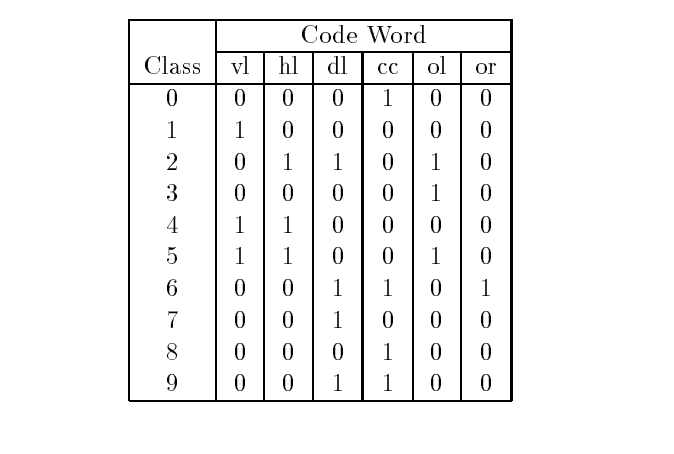
\includegraphics[bb=0 0 680 500,scale=.3]{FIG/code.png}
\caption{Coding scheme for 10 digits recognizing problem}
\end{figure}

The meaning of those codes follows the description in the figure 2 from \cite{Thomas1995}.


\begin{figure}[!htbp]
\centering
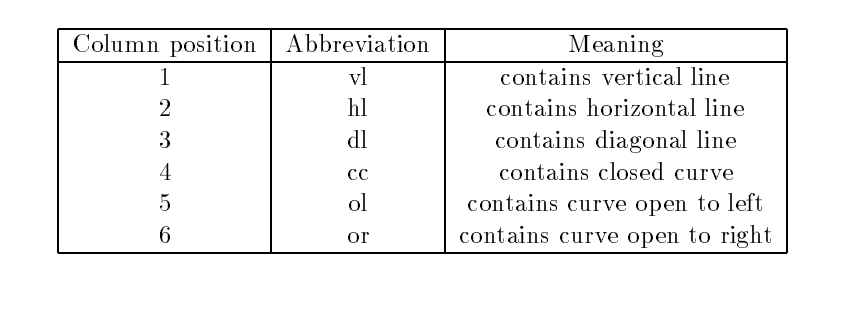
\includegraphics[bb=0 0 860 300,scale=.3]{FIG/meaning.png}
\caption{Meaning of each bit}
\end{figure}

There are basically two principles for design a code\cite{Thomas1995}:
\begin{enumerate}
    \item \textbf{Row Distance}: The hamming distance between each two classes' codes should be as large as possible to make classes more distinguishable from each other.
    \item \textbf{Column Distance}: Each bit classifier should be independent from each other.
\end{enumerate}

It is obvious that there is a trade-off between those two principles, which leads to different code design methods. We will adapt the one described in Thomas's Paper\cite{Thomas1995}, which is every effective to generate compact yet distinguish code.

\subsubsection*{Running Fast BP for Bits}

As we already described in the previous sections, after designing of code, we run Fast BP for each bits, note as $f_{1}...f_{n}$. We can interpret $f_{i}(x)$ as the probability that the number appear on the $i^{th}$ bit of the code for a given example $x$ is 1.

\subsubsection*{Deciding Label}

For a node $r$, after computation, we get a vector of predictions of those functions:

\begin{gather*}
    f(r) = (f_{1}(r)...f_{n}(r))
\end{gather*}


In order to make final prediction we should find the class which is \textit{closest} to $f(r)$.

In general, there are different approaches to achieve this:

\begin{enumerate}
    \item \textbf{Hamming Decoding}: Transform $f(r)$ from real-value to binary value, and calculate the Hamming distance with code of each class. The label that has the shortest hamming distance is chosen.
    \item \textbf{Loss-based Decoding}: This method is introduced in \cite{Erin2000}, which defines a loss function between probability made by $f$ and the target bit of class, without transform $f(r)$ into binaries.
\end{enumerate}

\subsubsection*{Practical Variations of ECOC}

Error correcting code suffers from one major disadvantage, that is, if the number of classes is large, the number of bits will grow excessively, even exponentially. Sometimes, if the classification algorithm itself is time-consuming, such as Fast BP, even the number of bits is reasonable, ECOC becomes very expensive.

So we introduce a practical variation of ECOC, called One-VS-All schema. In \cite{Erin2000}, One-VS-All is proved to be a special case of ECOC.

It follows a very simple strategy: for every class, we train a binary classifier to distinguish whether a node is a class or not. The decision of final label is simple too, we just pick the class that has the highest $YES$ probability. One-VS-All will significantly reduce the number of bits involved, especially when $k$ is large. And as \cite{Ryan2000} suggests, when the underlying binary classifier performs well, One-VS-All works as well as ECOC approach.

%\begin{enumerate}
%   \item \textbf{One-Vs-All}: In this scheme every class is associated with a classifier that tells whether an incoming example is in this class or not. The final prediction is made according to some predefined decision value, like probability given by Logistics Regression.
%   \item \textbf{All-Vs-All}: A classifier is trained for every pair of classes. As there are $O(n^{2})$ classifiers to train, some algorithms are introduced to reduce the number of classifier pairs\cite{Platt2000}
%\end{enumerate}

Actually, the two schemes are just special case of ECOC, but are much more straight forward.


\subsection{FastBP for Multiple Classes}
The original Belief propagation update rules are as follows:

\begin{equation}
\label{eq:origbp_b}
b_i(x_k) = \eta\cdot \phi_i(x_k)\cdot\mathop{\prod}_{j\in N(i)}m_{ji}(x_k)
\end{equation}
\begin{equation}
\label{eq:origbp_m}
m_{ij}(x_g)=\mathop{\sum}_{x_k}\phi_{i}(x_g)\cdot \psi_{ij}(x_k,x_g)\cdot\mathop{\prod}_{n\in N(i)\setminus j} m_{ni}(x_k)
\end{equation}

where $x_k$ is one state for any node and $b_i(x_k)$ is the probability (belief) for node $i$ staying at state $x_k$. So the first step of approximating the original rules is to remove the product operators. A very intuitive and common method is taking logarithms of both sides. For Eq.(\ref{eq:origbp_b}), it becomes
\begin{equation}
\log(b_i(x_k)) = \log(\eta) + \log(\phi_i(x_k)) + \mathop{\sum}_{j\in N(i)}\log(m_{ij}(x_k))
\end{equation}

Like the work~\cite{KoutraKKCPF11} by Koutra, et al., we have to use a smart approximation for the logarithm. But let us skip this part for a moment. Assume we have a reasonable approximation of logarithms now, i.e. $F(v)\approx \log(v)$, if $v$ is a vector, then $F(v)$ is also a vector whose each component is the approximation of the logarithm of corresponding $v$'s component.

So we can rewrite Eq.(\ref{eq:origbp_b}) as $F(b_i(x_k))=C_{ik}+\mathop{\sum}_{j\in N(i)}F(m_{ij}(x_k))$, where $C_{ik}=\log\eta + \log(\phi_i(x_k))$. Moreover, we use $\mathbf{b_i}$ as the status vector of beliefs of node $i$. For simplicity, assume there are only three classes, $x_k\in \{x_1, x_2, x_3\}$, i.e. $\mathbf{b_i} = \left[ \begin{array}{c}
b_i(x_1) \\
b_i(x_2) \\
b_i(x_3) \end{array} \right]$ we can get the general equation for any node $i$,

\begin{equation}
F(\mathbf{b_i})=
\left( \begin{array}{cccc}
F(\mathbf{m_{i1}})&F(\mathbf{m_{i2}})&\cdots& F(\mathbf{m_{in}})\end{array} \right)\mathbf{A_i}+\mathbf{C_i}
\end{equation}

where $\mathbf{A_i}$ is the $i$th column of the adjacency matrix and $\mathbf{C_i} = \left[ \begin{array}{c}
C_{i1} \\
C_{i2} \\
C_{i3} \end{array} \right]$
and $\mathbf{m_{ij}} = \left[ \begin{array}{c}
m_{ij}(x_1) \\
m_{ij}(x_2) \\
m_{ij}(x_3) \end{array} \right]$, Now, replace $\phi_i(x_k)\prod_{n\in N(i)\setminus j} m_{ni}(x_k)$ with $b_i(x_k)/(\eta m_{ji}(x_k))$, Eq.(\ref{eq:origbp_m}) can be rewritten as $m_{ij}(x_k) = \sum_{x_g}\psi_{ij}(x_k,x_g)b_i(x_k)/(\eta m_{ji}(x_k))$, which means
\begin{equation}
\mathbf{m_{ij}} = \frac{1}{\eta} \Psi_{ij} \left[ \begin{array}{c}
b_i(x_1)/m_{ji}(x_1) \\
b_i(x_2)/m_{ji}(x_2) \\
b_i(x_3)/m_{ji}(x_3) \end{array} \right]
\end{equation}


where $\Psi$ is the correlation (transition) matrix of every two nodes, i.e., under the three class assumption,
\begin{equation}
\Psi_{ij} = \left[ \begin{array}{ccc}
\psi_{ij}(x_1,x_1)&\psi_{ij}(x_1,x_2)&\psi_{ij}(x_1,x_3) \\
\psi_{ij}(x_2,x_1)&\psi_{ij}(x_2,x_2)&\psi_{ij}(x_2,x_3) \\
\psi_{ij}(x_3,x_1)&\psi_{ij}(x_3,x_2)&\psi_{ij}(x_3,x_3) \end{array} \right]
\end{equation}

It can also be written as
\begin{equation}
\mathbf{m_{ij}} = \frac{1}{\eta} \Psi_{ij} \left[ \begin{array}{ccc}
1/m_{ji}(x_1)&0&0 \\
0 &1/m_{ji}(x_2)&0 \\
0& 0 &1/m_{ji}(x_3) \end{array} \right] \left[ \begin{array}{c}
b_i(x_1)\\
b_i(x_2)\\
b_i(x_3)\end{array} \right]
\end{equation}

Suppose all nodes are homogeneous, i.e. $\forall i,j$ , $\Psi_{ij} = \Psi$ is non-singular (which is also the common case), then we get a relation between the state of one node and two different direction messages on its one edge (since $\eta$ is just a normalization constant, we ignore $\eta$ in the following analysis):
\begin{equation}
\mathbf{b_i} = diag(\mathbf{m_{ji}})\Psi^{-1}\mathbf{m_{ij}}
\end{equation}

Finally, we get the matrix equations for belief propagation,
\begin{equation}
\label{equ:bfnewrule_b}
\mathbf{b_i} = diag(\mathbf{m_{ji}})\Psi^{-1}\mathbf{m_{ij}}~~~~\forall i\in [n],~j\in N(i)
\end{equation}

\begin{equation}
\label{equ:bfnewrule_m}
F(\mathbf{b_i})=
\left( \begin{array}{cccc}
F(\mathbf{m_{i1}})&F(\mathbf{m_{i2}})&\cdots& F(\mathbf{m_{in}})\end{array} \right)\mathbf{A_i}+\mathbf{C_i}~~~\forall i\in [n]
\end{equation}

\subsubsection{Simple correlation matrix case}

In many cases, one node is inclined to connect with other nodes which are in the same class as itself. For example, when we buy a book in Amazon, it is very possible that we also buy another book, which has close relation with the first one (e.g. supplementary textbook), or the one that is suggested by the suggestion system. Another instance is that when we post a scenery photo on facebook, it is very likely that at the same time you will post more scenery photos instead of other kinds of photos. Based on this fact, we assume a simple case that the correlation matrix is almost as an identity matrix. In this case, $\Psi^{-1} \approx \mathbf{I}$, then

\begin{equation}
\label{equ:simplecorrelation}
\mathbf{b_i} \approx diag(\mathbf{m_{ji}})\mathbf{m_{ij}} = \mathbf{m_{ji}}\circ \mathbf{m_{ij}}
\end{equation}

where ``$\circ$'' is the hadamard product (element-wise product). However, the identity correlation matrix has a problem: if the graph is a strong connected graph, there is no feasible solution exists according to Eq.(\ref{equ:simplecorrelation}), since all the nodes are connected and they can only all belong to the same class. To avoid this problem, we allow the deviation for all beliefs,
$$\mathbf{b_i}  \leq \mathbf{m_{ji}}\circ \mathbf{m_{ij}} + \mathbf{s_i}$$
and $\mathbf{s_i} \geq 0$, i.e. every entry of $\mathbf{s_i}$ is greater than $0$. But put penalty on these slack variables. Also note that $\mathbf{m_{ij}}$ and $\mathbf{m_{ji}}$ always come in pairs, we can use $\mathbf{m'_{ij}} ~(= \mathbf{m'_{ji}})$ to replace $\mathbf{m_{ji}}\circ \mathbf{m_{ij}} ~(= \mathbf{m_{ij}}\circ \mathbf{m_{ji}})$, so basically we need to solve this optimization problem,
\begin{equation}
\begin{aligned}
& \underset{\mathbf{s}}{\text{minimize}}
& & \frac{1}{2}\mathop{\sum}_{k \in [n]\setminus V_0, j\in N(k)}||\mathbf{b_k} - \mathbf{m'_{kj}}||^2 + \lambda \sum_i^n\mathbf{s_i} \\
& \text{subject to}
& &  \mathbf{b_i}-\mathbf{s_i} \leq \mathbf{m'_{ij}}, ~~\; i \in V_0, j\in N(i)\\
& &  &\mathbf{b_k}-\mathbf{s_k} \leq \mathbf{m'_{kj}}, ~~\; k \in [n]\setminus V_0, j\in N(k)\\
& &  &\mathbf{s_i}\geq 0 ~~\; i \in [n]\\
& &  &\mathbf{b_i}\geq 0 ~~\; i \in [n]\setminus V_0\\
& &  &\mathbf{m'_{ij}}\geq 0 ~~\; i \in [n], j\in N(i)
\end{aligned}
\end{equation}
Note that the node set $V_0$ is the labeled node set, i.e. $\mathbf{b_i}$, $i\in V_0$ is given. $\lambda$ is the adjustable weight which determines the importance of the deviation in our final result and remember $\mathbf{m'_{ij}} = \mathbf{m'_{ji}}$. If we want more initial labeled nodes can fit in this model, then give a larger value to $\lambda$, but meanwhile the estimation of the target nodes' beliefs tend to become worse. There are many methods to solve this standard optimization problem. We just give an example with Karush-Kuhn-Tucker (\textbf{KKT}) conditions which finally winds up into an equation system.

Add lagrangian multiplier $\alpha_{ij} \geq 0$, $\beta_i \geq 0$, $\mu_i \geq 0$ and $\nu_i\geq 0$, $i\in V_0$, $j\in N(i)$  here, we get

\begin{align*}
&\frac{1}{2}\mathop{\sum}_{k \in [n]\setminus V_0, j\in N(k)}||\mathbf{b_k} - \mathbf{m'_{kj}}||^2 + \lambda\sum_i^n\mathbf{s_i} + \mathop{\sum}_{i=1}^n\alpha_{ij}(\mathbf{b_i}
-\mathbf{s_i} -  \mathbf{m'_{ij}}) \\&- \sum_{i\in [n]} \beta_{i}\mathbf{s_i} - \sum_{i\in [n]\setminus V_0} \mu_{i}\mathbf{b_i} - \sum_{i\in [n], j\in N(i)} \nu_{i}\mathbf{m'_{ij}}
\end{align*}



It is easy to see that this optimization problem is a convex optimization problem, but we also need to assume there are positive feasible solution (i.e. strong convexity of optimization problem). Then according to the \textbf{KKT} conditions, we can get the global optimal solution.
\begin{align}
\label{equ:kkt1}
&\mathbf{b_k} - \mathbf{m'_{kj}} - \mu_k\vec{1} = 0 ~~~~&\forall k\in [n]\setminus V_0, j\in N(k)\\
\label{equ:kkt2}
&- \mathbf{b_k} + \mathbf{m'_{kj}} - \alpha_{jk}\vec{1} - \nu_{k}\vec{1} = 0 &\forall k\in [n]\setminus V_0, j\in N(k)~~and~~j\in V_0\\
\label{equ:kkt3}
&- \mathbf{b_k} - \mathbf{b_j} + 2\mathbf{m'_{kj}} - \nu_{k}\vec{1} = 0 &\forall k\in [n]\setminus V_0, j\in N(k)~~and~~j\in [n]\setminus V_0\\
\label{equ:kkt4}
& \alpha_{ij} = \alpha_{ji} = 0 &\forall i\in V_0, j\in N(i)~~and~~j\in V_0\\
\label{equ:kkt5}
&\lambda - \sum_{j\in N(i)}\alpha_{ij}\vec{1} - \beta_i \vec{1}=0 &\forall i\in V_0\\
\label{equ:kkt6}
&\alpha_{ij}(\mathbf{b_i}-\mathbf{s_i}- \mathbf{m'_{ij}}) = 0 &\forall i\in V_0, j\in N(i)\\
\label{equ:kkt7}
&\beta_i \mathbf{s_i} = 0 &\forall i\in V_0\\
\label{equ:kkt8}
&\mu_i \mathbf{b_i} = 0 &\forall i\in [n]\setminus V_0\\
\label{equ:kkt9}
&\nu_i \mathbf{m'_{ij}} = 0 &\forall i\in V_0, j\in N(i)
\end{align}

Even though it seems very complicated, all of these equations are very simple, and we need all of these equations to get the optimal result.  Eq.(\ref{equ:kkt1})$\sim$ Eq.(\ref{equ:kkt4}) are from the stationary condition of \textbf{KKT} condition, which describe the relationship between any two nodes (there are three kinds of node pair $(i,j)$ (1) $i,j$ are both labeled nodes in $V_0$, ; (2) one of $i,j$ is labeled node and another one is the target node; (3) $i,j$ are both target nodes. The belief results are all $\mathbf{b_k}$, $k\in [n]\setminus V_0$.

\subsubsection{Extended correlation matrix case}

Before we talk about the common correlation matrix, we should think about why the optimization problem proposed above works. See Fig.~\ref{fig:bpexample} for an example part of a small \textbf{BP} network. The idea of the previous optimization problem comes from ignoring the real value of the $m_{ij}$ and $m_{ji}$, but using a generalized variable $m'_{ij}$ to describe the relationship between two nodes $i$ and $j$.

Assume node $i$ is a labeled node, i.e. $\mathbf{b_i}$ is known, according to last subsection, the value of $\mathbf{m'_{ij}}$ can be bounded by $\mathbf{b_i}$ and $\mathbf{s_i}$. On the other hand, if node $j$ is an unknown (target) node, $\mathbf{b_j}$ can also be bounded by $\mathbf{m'_{ji}}$ and $\mathbf{s_j}$. The key point here is that $\mathbf{m'_{ij}} = \mathbf{m'_{ji}}$. This equation means we can approximate $\mathbf{b_j}$ with $\mathbf{b_i}$, $\mathbf{s_i}$ and $\mathbf{s_j}$. $\mathbf{s_i}$ and $\mathbf{s_j}$ are just the slack variables we defined, and we minimize all the slack variables in the objective functions. In one word, the captured relation between $\mathbf{m'_{ij}}$ and $\mathbf{m'_{ji}}$ can be used to describe the relation between $\mathbf{b_i}$ and $\mathbf{b_{j}}$, which is the objective to be optimized.

\begin{figure}[!htb]
\begin{center}
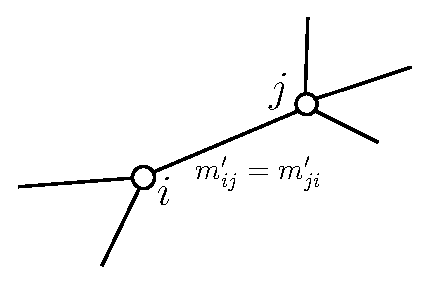
\includegraphics[scale=0.8]{FIG/bpexample}
{\caption{Small example of BP network}\label{fig:bpexample}}
\end{center}
\end{figure}

Recall that we actually use $\mathbf{m'_{ij}}$ to replace $diag(\mathbf{m_{ji}})\Psi^{-1} \mathbf{m_{ij}}$. Obviously that $\mathbf{m'_{ij}} = \mathbf{m'_{ij}}$ does not hold for common correlation matrix $\Psi$. But if we have

$$\mathbf{m'_{ij}} \approx \mathbf{m'_{ji}}$$
which holds in some cases, for instance that if $\Psi$ is close to $\mathbf{I}$. This assumption means that the analysis in the simple correlation matrix case still works. Also, we need to think about that why the slack variables $\mathbf{s_i}$, $i\in [n]/V_0$ are necessary. Simply speaking, the main reason is that we just use Eq.(\ref{equ:bfnewrule_b}) without Eq.(\ref{equ:bfnewrule_m}) to formulate the optimization problem. Although Eq.(\ref{equ:bfnewrule_b}) is derived by substituting $\phi_i(x_k)\prod_{n\in N(i)\setminus j} m_{ni}(x_k)$ with $b_i(x_k)/(\eta m_{ji}(x_k))$, which comes directly from Eq.(\ref{equ:bfnewrule_m}), we still lose parts of all the information of the original belief updating rule.

Due to the limitation of time, there are still two unsolved problems which can be interesting topics for further study. The first one is that we provide an equation system which is used to solve the optimization problem. How to organize these equations into a more concise form is not a easy task. The second problem, how can we derive an upper bound for the distance between the solution to the optimization problem and the solution of the original Belief Propagation algorithm. For example, if we are given $||\mathbf{m'_{ij}} - \mathbf{m'_{ji}}||_F^2 \leq \epsilon$, (here is the componentwise norm, i.e. Frobenius norm), we hope to derive an error upper bound as a function of $\epsilon$. Since we do not have time to implement some experiments to test the accuracy of this method, testing this result on different networks may be the next step.

\subsubsection{Quadratic approximation}
We also try another direction (relaxing the approximation assumption) to extend the \textbf{FaBP}, even though we do not really figure it out. A significant fact of the original \textbf{FaBP} algorithm is the assumption that all parameters are ``about half'', i.e. close to 1/2. This assumption provides a foundation for the correctness of Maclaurin series expansion used in the analysis. However, when there are more than two classes, without the concept of odd-ratio, we cannot achieve the similar assumption for any parameter. But we can use the quadratic approximation, i.e. second order Taylor approximation for the logarithms, i.e. instead of using $\log(x) \approx \log(1)+\log^{\prime}(1)(x-1)$ with the assumption that $x$ (the odd-ratio) is close to $\frac{1}{2}$, we use
$$\log(x)\approx \log(1)+\log^{\prime}(1)(x-1)+\frac{\log^{\prime\prime}(1)}{2}(x-1)^2$$
without the ``about half'' assumption.

More precisely, in Eq.(\ref{equ:bfnewrule_m}), $F(v) = (v - 1) - \frac{(v -1)^2 }{2}$

Still, for simplicity we assume there are three states for the node, i.e. $x_k\in \{x_1, x_2, x_3\}$. Then the left hand side of Eq.~(\ref{equ:bfnewrule_m}) is
\begin{equation}
\left[ \begin{array}{c}
b_i(x_1) \\
b_i(x_2) \\
b_i(x_3) \end{array} \right]
\circ
\left[ \begin{array}{c}
2-\frac{1}{2}b_i(x_1) \\
2-\frac{1}{2}b_i(x_2)\\
2-\frac{1}{2}b_i(x_3)\end{array} \right]
-
\left[ \begin{array}{c}
\frac{1}{2} \\
\frac{1}{2} \\
\frac{1}{2} \end{array} \right]
=
diag(\mathbf{b_i})(
\left[ \begin{array}{c}
2\\
2\\
2\end{array} \right]
-\frac{1}{2}\mathbf{b_i})
-
\left[ \begin{array}{c}
-\frac{1}{2} \\
-\frac{1}{2} \\
-\frac{1}{2} \end{array} \right]
\end{equation}

note that
\begin{equation}
diag(\mathbf{b_i}) \vec{\mathbf{1}}= \left[ \begin{array}{ccc}
b_i(x_1)&0&0 \\
0&b_i(x_2)&0 \\
0&0&b_i(x_3) \end{array} \right]\vec{\mathbf{1}}= \mathbf{b_i}
\end{equation}

Finally we get
\begin{equation}
\label{eq:newquadraticapprox}
diag(\mathbf{b_i})
(2\cdot\vec{\mathbf{1}}
-\frac{1}{2}\mathbf{b_i})-
\frac{1}{2}\vec{\mathbf{1}}
= \left( \begin{array}{cccc}
\mathbf{M_{i1}}&\mathbf{M_{i2}}&\cdots& \mathbf{M_{in}}\end{array} \right)\mathbf{A_i}+\mathbf{C_i}
\end{equation}

where $\mathbf{M_{ij}}$ can also be written as
$diag(\mathbf{m_{ij}})(2\cdot \vec{\mathbf{1}}-\frac{1}{2}\mathbf{m_{ij}})-\frac{1}{2}\vec{\mathbf{1}}$.

This new equation is still very complicated. But since the ``about-half'' assumption has been removed from this updating rule, it also has potential to be used in formulating a optimization problem as we discussed in previous sections, and if it can be done, the accuracy of the optimization problem will be definitely improved. Even though we cannot find a good usage for this new approximation of the belief updating rule now, we still believe it is an attemptable research point.




\section{Experiments}
    \label{sec:experiments}
     \subsection{Preliminary Experiments}
We did some preliminary experiments on BP and FastBP algorithms.

By extracting all the items, whose groups are DVD, Video and Music from the Amazon co-purchase dataset, we get 149,102 nodes and 253,407 edges connecting them.
The classification accuracy of BP is around 72\% with 5\% nodes labeled.

We then reduced the dataset to just two types (DVD and Video) of items and run FastBP on it.
The result shows that there are only 4,274 nodes have non-zero bias from 50\% probability to either type (2,298 (5\%)of them have prior value) after 10 iterations.


%\section{Conclusions}
%    \label{sec:conclusions}
%    Pending


\bibliography{BIB/christosref,BIB/other}
\bibliographystyle{plain}

\newpage
\appendix
\section{Appendix}
\subsection{List of Innovations}
\bit
\item Evaluate BP and Fast BP on many real world datasets.
\item Improve BP on Hadoop with convergence detection.
\item Use ECOC to extend Fast BP to multiclass.
\item Use quadratic approximation to extend Fast BP to multiclass.
\eit

\subsection{Labor Division}

The team will perform the following tasks
\bit
\item Implementation of BP on Hadoop with convergence detection [Yu Su,Huanchen Zhang,1 weeks]
\item Parse data and build network from datasets mentioned above [All, almost done]
\item Evaluate BP and Fast BP on large graphs [All, already have preliminary results, 1 week]
\item Research on extending Fast BP algorithm to Multiclass Problem [Guanyu Wang,Yuchen Tian, 2 weeks]
\item Implement and evaluate multiclass Fast BP algorithm [Yu Su,Huanchen Zhang,1 weeks]
\eit

\subsection{Activities}
\bit
\item Guanyu Wang: Performed dataset analysis and network building. Read papers and tried to deduct quadratic approximation for FaBP extension.
\item Yuchen Tian: Performed dataset analysis and network building. Proposed error correcting code methods for FaBP extension.
\item Yu Su: Performed dataset analysis and network building. Did some preliminary experiments.
\item Huanchen Zhang: Performed dataset analysis and network building. Did some preliminary experiments.
\eit

\subsection{Previous Labor Division}

The team will perform the following tasks
\bit
\item Implementation of BP on Hadoop [Yu Su,Huanchen Zhang,2 weeks]
\item Apply BP on Large Graph [All,2 weeks]
\item Research on extending Fast BP algorithm to Multiclass Problem [Guanyu Wang,Yuchen Tian,2 weeks]
\eit



\newpage
\pagenumbering{roman}
\tableofcontents


\end{document}
